\documentclass[11pt]{article}

% ---------- Packages ----------
\usepackage[margin=1in]{geometry}
\usepackage{tikz}
\usetikzlibrary{arrows.meta, positioning, calc}
\usepackage{amsmath, amssymb}
\usepackage{booktabs}
\usepackage{graphicx}
\usepackage{caption}
\usepackage{hyperref}
\usepackage{times}
\usepackage{enumitem}

\title{The SDPNRI Compartmental Model of Rumour Spread\\
\large The influence of emotion contagion and political bias on debunkers threshold}
\author{}
\date{}

\begin{document}
\maketitle

\begin{abstract}
\textit{[Abstract to be added.]}
\end{abstract}

\section{Introduction}
\textit{[Introduction to be added.]}

\section{Methodology}

\subsection{The SDPNRI Compartmental Model}

For this research paper, an SDPNRI compartmental model was adopted to represent
different states for social media users (Susceptible, Doubtful, Positively-infected,
Negatively-infected, Restrained, Immune). This framework extends classical epidemic
modeling to capture the dynamics of rumour spread.

In social networks, the force of infection represents the per-capita rate at which an
individual encounters rumour-spreading content. Unlike real pathogens, which could
spread faster with a scaling susceptible density in a physical environment,
misinformation spread doesn't depend on the number of users but rather on network
topology, such as the number of followers and feed algorithms; intuitively, having a
bigger population doesn't imply having more social connections than in a smaller one.
Therefore, my model is frequency dependent.

In classical epidemiology frameworks, we assume homogeneous mixing and passive hosts,
where all individuals share identical properties and equal probabilities of
transitioning from one state to another. However, rumor dynamics are strongly
influenced by cognitive biases, polarities, and emotions. SDPNRI extends classic SIR
models by adopting behavioural and psychological phenomena that drive real-world
social networks dynamics.

\subsection{Model Compartments}

\begin{description}[leftmargin=2.2cm, style=nextline]
    \item[Doubtful] Represents individuals who, upon exposure, question the reliability
    of the information and express uncertainty until they either lose interest, commit
    to a polarised stance, or gain access to fact-checking sources.

    \item[Infection (P/N)] Physical pathogens typically infect hosts uniformly, while
    infection in social networks triggers different ideologies and affective
    responses. Positively-Infected users propagate the rumours with positive
    sentiments and endorsement, while Negatively-Infected users circulate the same
    rumour with negative emotions, outrage, and criticism. Recent studies show that
    negative news tends to spread faster than positive ones, which justifies this
    modeling decision.

    \item[Restrained] Represents people who, over time, lose interest in the rumour and
    stop spreading it or questioning it because of social-media fatigue.

    \item[Immune] Represents people with enough expertise to know that a rumour is
    false, or fact-checkers who consult reliable sources. The Immune state is
    absorbing, rendering all subsequent state transitions impossible.
\end{description}

\subsection{State Transition Diagram}

Figure~\ref{fig:directed_sdpnri} shows the directed state-transition graph for the
SDPNRI model.

\begin{figure}[htbp]
\centering
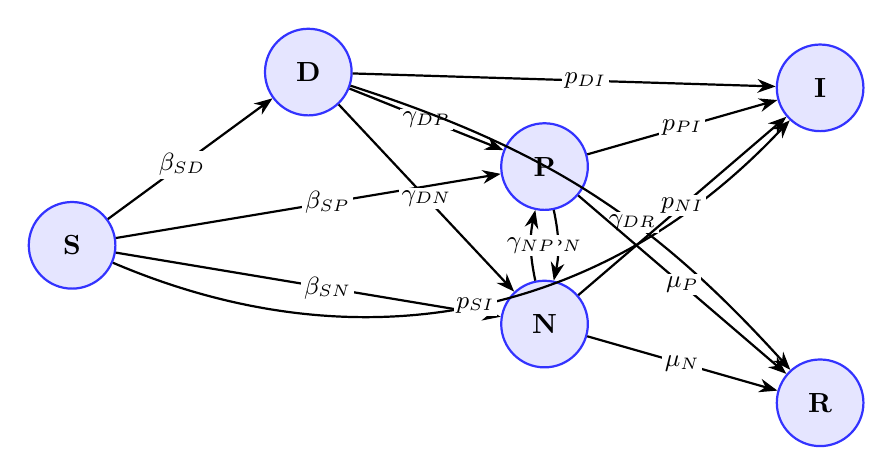
\begin{tikzpicture}[
    node/.style={circle, draw=blue!80, fill=blue!10, thick, minimum size=1.1cm, font=\bfseries},
    lbl/.style={font=\small, fill=white, inner sep=1pt},
    ->, >=Stealth, thick
]
    % Nodes (manual layered layout)
    \node[node] (S) at (0,0)     {S};
    \node[node] (D) at (3,2.2)   {D};
    \node[node] (P) at (6,1)     {P};
    \node[node] (N) at (6,-1)    {N};
    \node[node] (I) at (9.5,2)   {I};
    \node[node] (R) at (9.5,-2)  {R};

    % Edges from S
    \draw (S) -- node[lbl, pos=0.45] {$\beta_{SD}$} (D);
    \draw (S) -- node[lbl, pos=0.55] {$\beta_{SP}$} (P);
    \draw (S) -- node[lbl, pos=0.55] {$\beta_{SN}$} (N);
    \draw (S) to[bend right=35] node[lbl, pos=0.5] {$p_{SI}$} (I);

    % Edges from D
    \draw (D) -- node[lbl, pos=0.5] {$\gamma_{DP}$} (P);
    \draw (D) -- node[lbl, pos=0.5] {$\gamma_{DN}$} (N);
    \draw (D) -- node[lbl, pos=0.55] {$p_{DI}$} (I);
    \draw (D) to[bend left=15] node[lbl, pos=0.6] {$\gamma_{DR}$} (R);

    % Edges from P
    \draw (P) -- node[lbl, pos=0.5] {$p_{PI}$} (I);
    \draw (P) -- node[lbl, pos=0.5] {$\mu_{P}$} (R);

    % Edges from N
    \draw (N) -- node[lbl, pos=0.5] {$p_{NI}$} (I);
    \draw (N) -- node[lbl, pos=0.5] {$\mu_{N}$} (R);

    % Cross-infection between P and N (present in the ODE system)
    \draw (P) to[bend left=12] node[lbl, pos=0.5] {$\gamma_{PN}$} (N);
    \draw (N) to[bend left=12] node[lbl, pos=0.5] {$\gamma_{NP}$} (P);
\end{tikzpicture}
\caption{Directed state transition graph for the SDPNRI model.}
\label{fig:directed_sdpnri}
\end{figure}

\subsection{Governing Equations}

The system of ordinary differential equations describing the macro-level SDPNRI
dynamics is given by:

\begin{align*}
\frac{dS}{dt} &= -p_{SI}S - (\beta_{SD} + \beta_{SP} + \beta_{SN})S(P+N) \\[4pt]
\frac{dD}{dt} &= \beta_{SD}S(P+N) - (\gamma_{DP} + \gamma_{DN} + \gamma_{DR} + p_{DI})D \\[4pt]
\frac{dP}{dt} &= \beta_{SP}S(P+N) + \gamma_{DP}D - \mu_{P}P - p_{PI}P - \gamma_{PN}P + \gamma_{NP}N \\[4pt]
\frac{dN}{dt} &= \beta_{SN}S(P+N) + \gamma_{DN}D - \mu_{N}N - p_{NI}N - \gamma_{NP}N + \gamma_{PN}P \\[4pt]
\frac{dI}{dt} &= p_{SI}S + p_{DI}D + p_{PI}P + p_{NI}N \\[4pt]
\frac{dR}{dt} &= \gamma_{DR}D + \mu_{P}P + \mu_{N}N
\end{align*}

\begin{table}[htbp]
\centering
\caption{SDPNRI Model Transition Rates}
\label{tab:transition_rates}
\begin{tabular}{lc}
\toprule
\textbf{Rate} & \textbf{Transition} \\
\midrule
$p_{SI}$      & $S \rightarrow I$ \\
$\beta_{SD}$  & $S \rightarrow D$ \\
$\beta_{SP}$  & $S \rightarrow P$ \\
$\beta_{SN}$  & $S \rightarrow N$ \\
$\gamma_{DP}$ & $D \rightarrow P$ \\
$\gamma_{DN}$ & $D \rightarrow N$ \\
$\gamma_{DR}$ & $D \rightarrow R$ \\
$p_{DI}$      & $D \rightarrow I$ \\
$p_{PI}$      & $P \rightarrow I$ \\
$p_{NI}$      & $N \rightarrow I$ \\
$\mu_P$       & $P \rightarrow R$ \\
$\mu_N$       & $N \rightarrow R$ \\
\bottomrule
\end{tabular}
\end{table}

The system of ordinary differential equations presented above describes the
macro-level theoretical framework of the SDPNRI model in a homogenous approach,
assuming continuous population-level transmission rates. Therefore, to test and
validate this theoretical model against real-world social network dynamics --
including asynchronous user activities, political biases, and emotional contagion --
an Agent-Based Model (ABM) was created, calibrated using a real dataset.

\subsection{Dataset}

For this research paper, a subset of the PHEME-Aug (v1.0) augmented rumor dataset
published by Han, Gao, and Ciravegna (2019) was used. This corpus enhances the
original PHEME dataset for rumor detection (Kochkina et al., 2018) by adding
supplementary contextual threads from the CrisisLexT26 crisis repository (Olteanu et
al., 2015).

While PHEME-Aug covers multiple historical events, this study explicitly isolates the
sub-corpus tracking the 2013 Boston Marathon bombings only, specifically the rumour
that claimed the death of an 8 year-old girl at the Boston Marathon finish line while
running to raise money for the victims of the Sandy Hook Elementary School shooting
(which had occurred four months prior, in December 2012). The original story involved
an 8 year old boy named Martin Richard who was killed while cheering for his family
and friends near the finish line.

This data is extracted from Twitter, which was renamed ``X'' in 2023. It is a
microblogging platform that allows users to post personal content such as tweets, and
navigate a feed page driven by algorithms that prioritize recent content from people
they follow. It offers options to `retweet' posts, which would increase its reach and
spread it to the retweeter's network, or react to it through comments and likes. My
chosen dataset tracks twitter activities at the 2013 Boston bombings event, and it
includes text content, posting time, user\_id\ldots My ABM will simulate a closed
Twitter population ruled by transmission rates concluded from the calibration of my
dataset.

\subsection{Calibration of Transmission Rates}

To calibrate my transmission rates, I developed a computer program that extracts the
text across all activities in my dataset and feeds it to Claude AI to classify into
Infectious, Immune, Doubtful, and Irrelevant, using a well structured prompt where
Irrelevant represents activities that do not relate to the rumour topic. For
Infectious categories, VADER sentiment-analysis was used to classify the infectious
activities into Positively-Infected or Negatively-Infected based on the tonality of
the text. VADER is a lexicon-based tool designed to assign a compound score between
$-1$ (most extreme negative) and $+1$ (most extreme positive). Scores above $0.05$
mean positive, below $-0.05$ mean negative, and values in between mean neutral.

For the purpose of this study, neutral sentiment classification was omitted, and the
new threshold for negative classification was adjusted to below $-0.3$, which was
tested empirically, due to the high negative emotions that revolve around a child's
death rumour.

Because my data can not specify the exact moment a user becomes inactive, a 12-hour
duration of continuous inactivity following an agent's last recorded post was
operationalized as the transition threshold into the Restrained ($R$) compartment.
Recent studies demonstrate that over 60\% of crisis-related retweeting cascades
naturally cease diffusion within a 12-hour window as social media attention shifts
and information fatigue sets in (Li et al., 2021; Pfeffer et al., 2023).

\begin{figure}[htbp]
\centering
\includegraphics[width=0.85\textwidth]{figs/boston_bombings.png}
\caption{SDPNRI compartment dynamics over time, calibrated on the Boston Marathon
bombings dataset. $N = 482$.}
\label{fig:boston_bombings}
\end{figure}

The model updates compartment populations dynamically as a function of elapsed time
$t$ (measured in seconds since global $t_0$), as shown in Figure~\ref{fig:boston_bombings}.
Because individual agent activities are asynchronous, state transitions occur at
discrete empirical timestamps across the total population $N = 482$.

To calibrate the model transition parameters, empirical hazard rates were estimated
using the person-time incidence rate method. For each permitted transition from $A$ to
$B$, the rate per second was derived by dividing the total count of observed
transitions by the cumulative person-time exposure spent by agents in the source state
$A$ before transitioning to another state.

\begin{equation*}
\lambda_{A \to B} = \frac{N_{A \to B}}{\text{Exposure}_A}
= \frac{N_{A \to B}}{\sum_{i=1}^{M} A(t_i) \cdot \Delta t_i}
\end{equation*}

\begin{table}[htbp]
\centering
\caption{Empirically Calibrated Transition Rates}
\label{tab:calibrated_rates}
\begin{tabular}{lccc}
\toprule
\textbf{Transition} & \textbf{Events} & \textbf{Person-seconds} & \textbf{Rate per second} \\
\midrule
$D \to I$ & 2   & 1{,}229{,}508 & $1.6267 \times 10^{-6}$ \\
$D \to N$ & 0   & 1{,}229{,}508 & $0$ \\
$D \to P$ & 2   & 1{,}229{,}508 & $1.6267 \times 10^{-6}$ \\
$N \to D$ & 5   & 8{,}697{,}323 & $5.7489 \times 10^{-7}$ \\
$N \to I$ & 3   & 8{,}697{,}323 & $3.4493 \times 10^{-7}$ \\
$N \to P$ & 16  & 8{,}697{,}323 & $1.8396 \times 10^{-6}$ \\
$P \to D$ & 1   & 3{,}508{,}268 & $2.8504 \times 10^{-7}$ \\
$P \to I$ & 2   & 3{,}508{,}268 & $5.7008 \times 10^{-7}$ \\
$P \to N$ & 2   & 3{,}508{,}268 & $5.7008 \times 10^{-7}$ \\
$S \to D$ & 16  & 17{,}306{,}130 & $9.2453 \times 10^{-7}$ \\
$S \to I$ & 188 & 17{,}306{,}130 & $1.0863 \times 10^{-5}$ \\
$S \to N$ & 214 & 17{,}306{,}130 & $1.2366 \times 10^{-5}$ \\
$S \to P$ & 64  & 17{,}306{,}130 & $3.6981 \times 10^{-6}$ \\
\bottomrule
\end{tabular}
\end{table}

\subsection{Agent-Based Model}

Using the calibrated transmission rates above, I developed an agent based model with
the same exact properties of my previous population, and I received the results shown
in Figure~\ref{fig:abm_simulation}. The close alignment between both diagrams reflects
the reliability of person-time incidence rates in generating transmission rates that
mimic the real-world social networks dynamics.

\begin{figure}[htbp]
\centering
\includegraphics[width=0.85\textwidth]{figs/abm_simulation.png}
\caption{SDPNRI compartment dynamics over time from the Agent-Based Model simulation,
compared against the empirical Boston Marathon bombings data.}
\label{fig:abm_simulation}
\end{figure}

Rumour spread on social media depends on many factors, such as follower count,
activity levels, the age of the post, and the attractiveness of the post, which we
assume are all embedded within our calibrated transmission rates. However, to address
my research question regarding the effect of emotional contagion and political bias
in the immune compartment thresholds, adding a political bias is crucial to my ABM, as
the child's death rumour barely reflects any political bias but is rather heavily
driven by emotions. Political bias, in return, amplifies the emotion, whether through
outrage and criticism or endorsement and support. Therefore, I developed a theoretical
multiplier for the $S \to P$ and $S \to N$ transitions that shows how the transmission
rates will evolve and consequently affect other compartments as well.

\subsection{Political Bias and Emotional Contagion Extension}

The baseline emotional score of the post ($E_{\text{base}}$, derived from the
magnitude of the compound VADER score $\lvert S_{\text{vader}} \rvert$) is amplified
by the agent's political intensity, calculated as its distance from political
neutrality ($\text{Bias} = 1.0$). To account for the well-established bimodal nature
of affective polarization, where emotional arousal and transmission susceptibility
remain moderate near neutral stances but intensify toward ideological extremes
(Iyengar et al., 2019; Bail et al., 2018), this effective emotional activation
($E_{\text{effective}}$) is scaled by an emotional sensitivity exponent $e$, while the
overall susceptibility to state transitions across network agents is modulated by the
polarization sensitivity exponent $b$.

\begin{equation*}
E_{\text{effective}} = \left( E_{\text{base}} \times \left(1 + \left\vert \text{Bias} - 1.0 \right\vert\right) \right)^{e}
\end{equation*}

Where:
\begin{itemize}
    \item $\text{Bias} \in (0, 2]$ represents the agent's political ideology ($1.0$
    being strictly neutral).
    \item $e$ dictates how non-linearly emotional intensity scales transition rates.
\end{itemize}

\begin{figure}[htbp]
\centering
\includegraphics[width=0.75\textwidth]{figs/fig_emotional_curve.png}
\caption{Non-Linear Emotional Amplification Curve.}
\label{fig:emotional_curve}
\end{figure}

To determine whether the user is inclined to spread the rumour with positive or
negative sentiments, unnormalized directional weights $w_P$ and $w_N$ were computed.
The political bias sensitivity exponent ($b$) governs the strength of ideological
confirmation bias, non-linearly scaling how strongly an agent's political position
influences their engagement framing:

\begin{align*}
w_P &= E_{\text{effective}} \times (\text{Bias})^b \\
w_N &= E_{\text{effective}} \times \left(\frac{1}{\text{Bias}}\right)^b
\end{align*}

Finally, the baseline available probability pool $\beta_{PN}$ is partitioned
proportionally between the two states, ensuring that
$P(S \rightarrow P) + P(S \rightarrow N) \le \beta_{PN}$, with

\begin{equation*}
\beta_{PN} = \beta_0 \times \left(1 + \left\vert \text{Bias} - 1.0 \right\vert\right)^b
\end{equation*}

\noindent and

\begin{equation*}
\beta_0 = P(S \rightarrow N) + P(S \rightarrow P) \approx 1.606367 \times 10^{-5}
\end{equation*}

\begin{align*}
P(S \rightarrow P) &= \beta_{PN} \times \left( \frac{w_P}{w_P + w_N} \right) \\
P(S \rightarrow N) &= \beta_{PN} \times \left( \frac{w_N}{w_P + w_N} \right)
\end{align*}

\section{Results}

\subsection{R0 and Epidemic Thresholds}

\begin{figure}[htbp]
\centering
\includegraphics[width=0.85\textwidth]{figs/fig_peak_attack_rate.png}
\caption{Rumor Peak Attack Rate vs.\ Debunker Rate ($p_{SI}$) with $R_0 \le 1.0$
Threshold.}
\label{fig:peak_attack_rate}
\end{figure}

\begin{figure}[htbp]
\centering
\includegraphics[width=0.85\textwidth]{figs/fig_72hr_polarization.png}
\caption{72-Hour SDPNRI Compartment Dynamics across Polarization Levels (Debunker
Rate $p_{SI} = 3.8\%$).}
\label{fig:72hr_polarization}
\end{figure}

\begin{figure}[htbp]
\centering
\includegraphics[width=0.75\textwidth]{figs/fig_critical_threshold.png}
\caption{Critical Debunker Threshold ($l^{*}$) as a Function of Political Bias ($b$).}
\label{fig:critical_threshold}
\end{figure}

\begin{figure}[htbp]
\centering
\includegraphics[width=0.85\textwidth]{figs/fig_72hr_r0_threshold.png}
\caption{72-Hour SDPNRI Compartment Dynamics at Theoretical $R_0 \le 1.0$ Debunker
Intervention Rates.}
\label{fig:72hr_r0_threshold}
\end{figure}

\section*{References}


\end{document}
